\documentclass[a4paper]{article}
\usepackage[utf8x]{inputenc}
\usepackage[T1,T2A]{fontenc}
\usepackage[russian]{babel}
\usepackage{hyperref}
\usepackage{indentfirst} % включить отступ у первого абзаца
\usepackage{listings}
\lstset{inputpath=../listings}
\usepackage{color}
\usepackage{here} 
\usepackage{graphicx}
\graphicspath{{pics/}}

\usepackage{caption}
\renewcommand{\lstlistingname}{Листинг}

\usepackage{listings}
\lstdefinestyle{base_listing}{ %
extendedchars=\true,
basicstyle=\footnotesize,       % the size of the fonts that are used for the code
numbers=left,                   % where to put the line-numbers
numberstyle=\footnotesize,      % the size of the fonts that are used for the line-numbers
stepnumber=1,                   % the step between two line-numbers. If it is 1 each line will be numbered
numbersep=5pt,                  % how far the line-numbers are from the code
backgroundcolor=\color{white},  % choose the background color. You must add \usepackage{color}
showspaces=false,               % show spaces adding particular underscores
showstringspaces=false,         % underline spaces within strings
showtabs=false,                 % show tabs within strings adding particular underscores
frame=single,           % adds a frame around the code
tabsize=2,          % sets default tabsize to 2 spaces
captionpos=b,           % sets the caption-position to bottom
breaklines=true,        % sets automatic line breaking
breakatwhitespace=false,    % sets if automatic breaks should only happen at whitespace
escapeinside={\%*}{*)},          % if you want to add a comment within your code
postbreak=\raisebox{0ex}[0ex][0ex]{\ensuremath{\color{red}\hookrightarrow\space}},
keepspaces = true
}

\lstdefinestyle{crs_bash}{
  style    = {base_listing},
  language = {bash}
}

\lstdefinestyle{crs_cpp}{
  style    = {base_listing},
  language = {C++}
}

\usepackage[left=2.5cm, top=2cm, right=2cm, bottom=2cm, nohead]{geometry}

\begin{document}
\begin{titlepage} % начало титульной страницы

\begin{center} % включить выравнивание по центру

\large Санкт-Петербургский Политехнический Университет Петра Великого\\
\large Институт компьютерных наук и технологий \\
\large Кафедра компьютерных систем и программных технологий\\[6cm]
% название института, затем отступ 4,5см

\huge Операционные системы и среды\\[0.5cm]
\large Отчет по лабораторной работе №8\\[0.1cm]
\large Средства синхронизации потоков и процессов в ОС Linux и
их применение\\[5cm]
\end{center}

\begin{flushright}
\begin{minipage}{0.5\textwidth}
\begin{flushright}
\textbf{Работу выполнил:}

Петров Владислав

{Группа:} 43501/4\\


\textbf{Преподаватель:} 

Душутина Елена Владимировна
\end{flushright}
\end{minipage} % конец врезки
\end{flushright} % конец выравнивания по левому краю

\vfill % заполнить всё доступное ниже пространство

\begin{center}

\large Санкт-Петербург\\
\large \the\year % вывести дату

\end{center} % закончить выравнивание по центру

\thispagestyle{empty} % не нумеровать страницу
\end{titlepage} % конец титульной страницы

\vfill % заполнить всё доступное ниже пространство


\section{Цель работы}
	Изучение средств синхронизации потоков и процессов в ОС семейства Linux и
их применение.
	
\section{Программа работы}
\begin{enumerate}
\item Привести собственные результаты выполнения предложенных программ и  их анализ. 
\item Модифицировать предложенное решение таким образом, чтобы «читатели» не имели  доступа к памяти по записи. 
\item Предложить  более  рациональное  решение  задачи  «читатели-писатель»,  используя другие  средства  синхронизации  или  их  сочетание.  Объяснить  и  подтвердить экспериментально улучшение характеристик взаимодействия.
\item Разработать  клиент-серверное  приложение  для  полной задачи  «читатели-писатели»  с собственной системой ограничений на доступ каждого «читателя» к информации.
\item  Разработать  программу «читатели-писатели»  для  сетевого  функционирования.  Для этого выбрать подходящие средства IPC и  синхронизации.
\item Предложить  программное  решение  задачи  «производители-потребители».  Разница  с предыдущей задачей – возможность модификации считываемых данных.
\item Решить   задачу   «обедающие   философы», обосновать выбранные средства синхронизации.
\end{enumerate}

\section{Ход работы}
	Лабораторная выполняется на физической машине со следующими характеристиками:
	\lstinputlisting[style=crs_bash]{../listings/uname}

\subsection{Создание двух потоков: потока – производителя и потока – потребителя}
	\textbf{Задание.} Создание двух потоков: потока – производителя и потока – потребителя.
Потоки разделяют целочисленный массив, в который заносятся производимые и извлекаются потребляемые данные. Для наглядности и контроля за происходящим в буфер помещается наращиваемое значение, однозначно идентифицирующее производителя и номер его очередной посылки.
Код должен удовлетворять трем требованиям:\begin{itemize}
\item потребитель не должен пытаться извлечь значение из буфера, если буфер пуст;
\item производитель не должен пытаться поместить значение в буфер, если буфер полон;
\item состояние буфера должно описываться общими переменными (индексами, счетчиками, указателями связанных списков и т.д.).
\end{itemize}
Задание необходимо выполнить различными способами, применив следующие средства синхронизации доступа к разделяемому ресурсу:
\begin{itemize}
\item Мьютексы;
\item Семафоры;
\end{itemize}
Программы должны предоставлять возможность завершения по таймеру либо по команде оператора.
\textbf{Решение.}
Структурируем программу так, чтобы по изменению одного константного значения можно было запускать программу для разных средств синхронизации. Для этого будем использовать прекомпиляцию
	\begin{lstlisting}[style=crs_cpp]
#define TYPE_OF_SYNCHRONISE 1
enum //описание значений
{
	MUTEX = 0,
	SEM = 1,
	CRS = 2,
	EVENT =  3,
	COND =4
};
	\end{lstlisting}
	В нашем случае используются только два первых константных значения: 0 и 1
Данные параметры загружаются в структуру вида:
	\begin{lstlisting}[style=crs_cpp]
struct Configuration 
{ 
int numOfReaders; //число потоков-читателей 
int numOfWriters; //число потоков-писателей 
int sizeOfQueue;  //размер очереди 
int readersDelay; //задержка на работу читателей (в миллисек) 
int writersDelay; //задержка на работу писателей (в миллисек) 
int ttl; //"время жизни" 
};
	\end{lstlisting}
Вся конфигурационная информация загружается из файла, имеющего следующий вид:

	\begin{lstlisting}[style=crs_cpp]
NumOfReaders= 10 
ReadersDelay= 100 
NumOfWriters= 10 
WritersDelay= 200 
SizeOfQueue= 10 
ttl= 3
	\end{lstlisting}
Очередь определяется в виде структуры:
	\begin{lstlisting}[style=crs_cpp]
struct FIFOQueue //FIFO очередь 
{ 
char **data; 	//массив сообщений 
int writeindex; //индекс записи 
int getindex; 	//индекс чтения 
int size; 		//размер очереди 
short full; 	//очередь заполнена 
};
	\end{lstlisting}

	Результат выполнения программы приведен на рисунке \ref{img:alg_main_thread}.
	\begin{figure}[h!]
		\center{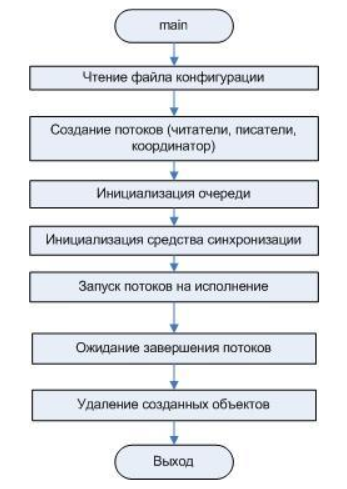
\includegraphics[scale=0.8]{alg_main_thread}}
		\caption{Схема алгоритма работы главного потока}
		\label{img:alg_main_thread}
	\end{figure}

	Исходный код функции главного потока:
	\lstinputlisting[style=crs_bash]{../listings/m_thread.c}
	Для структурирования кода использованы вспомогательные функции.
Функция SetConfig – производит чтение конфигурационного файла и заполнение структуры config. Функция CreateAllThreads – создает все потоки (читатели, писатели, координатор).\\

Исходный код вспомогательных функций:
	\lstinputlisting[style=crs_cpp]{../listings/assist.c}
	
	Схема алгоритма работы потока-координатора представлена на рис \ref{img:thr_coord}.
	\begin{figure}[h!]
		\center{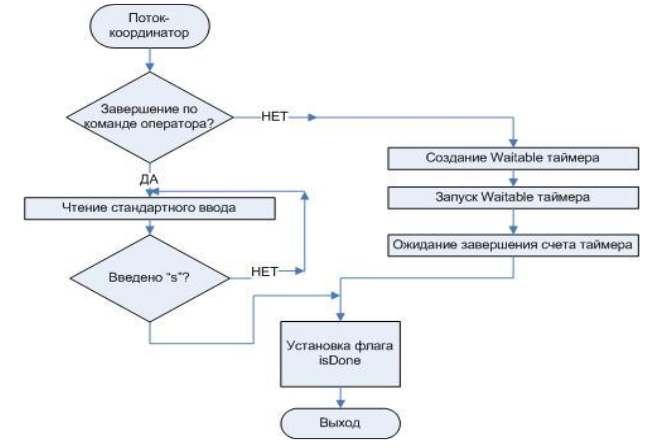
\includegraphics[scale=0.8]{thr_coord}}
		\caption{Схема алгоритма работы потока-координатора}
		\label{img:thr_coord}
	\end{figure}
	
	Исходный код функции потока-координатора:
	\lstinputlisting[style=crs_cpp]{../listings/coord.c}

	Схема алгоритма работы потока-читателя представлена на рис \ref{img:thr_reader}.
	\begin{figure}[h!]
		\center{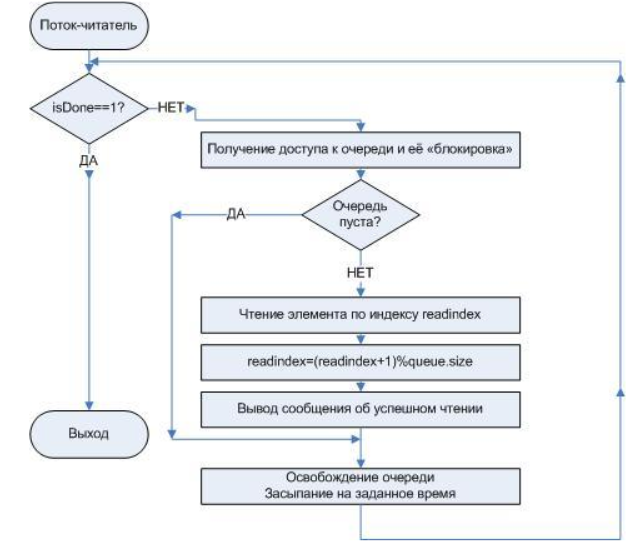
\includegraphics[scale=0.8]{thr_reader}}
		\caption{Схема алгоритма работы потока-читателя}
		\label{img:thr_reader}
	\end{figure}
	Исходный код потока-читателя:
	\lstinputlisting[style=crs_bash]{../listings/reader.c}
	Программа готова к запуску, необходимо лишь изменять константное значение.
	В дальнейшем используется следующая конфигурация:
	\begin{lstlisting}[style=crs_cpp]
NumOfReaders= 3 
ReadersDelay= 1 
NumOfWriters= 4 
WritersDelay= 1 
SizeOfQueue= 5 
ttl= 3
	\end{lstlisting}



\section{Вывод}
	
	

\end{document}

